\documentclass[a4paper,12pt,twoside]{book}
\usepackage[T1]{fontenc}
\usepackage[utf8]{inputenc}
\usepackage{lmodern}
\usepackage[english,french]{babel}
\usepackage{xspace} % pour la gestion des espaces après les commandes
\usepackage{xcolor}
\usepackage{minted} % colored source code
\usepackage{csquotes}
\usepackage{soul}

% Mise en page École des chartes
\usepackage[margin=2.5cm]{geometry} % marges
\usepackage{setspace}
\onehalfspacing % interligne de 1.5
\setlength\parindent{1cm}

\usepackage{tocbibind}
\usepackage[backend=biber, sorting=nyt, style=enc, minbibnames=10, maxbibnames=10]{biblatex}
\addbibresource{bibliographie/biblio_astro.bib}
\nocite{*}
\defbibnote{intro}{Cette bibliographie présente toutes les ressources utilisées, de tout type, citées ou non, par simple ordre alphabétique.}

\usepackage[pdfusetitle, pdfsubject={Mémoire TNAH — Titre}, pdfkeywords={mot1, mot2, mot3}]{hyperref}

\usepackage{graphicx}
\usepackage{subcaption}

\author{Prénom Nom – M2 TNAH — ENC}
\title{Titre mémoire}

% ACRONYMS
\usepackage[automake, acronym, toc]{glossaries}
\makeglossaries
\setacronymstyle{short-long}
\newacronym{fair}{\textsc{fair}}{\emph{Findable Accessible Interoperable Reusable}}
\newacronym{api}{\textsc{api}}{\emph{Application Programming Interface}}
\newacronym{eida}{EIDA}{Editing and analysing hIstorical astronomical Diagrams with Artificial intelligence}

% COMMANDS
\newcommand{\enc}{École nationale des chartes\xspace}
\newcommand{\fair}{\gls{fair}\xspace}
\newcommand{\api}{\gls{api}\xspace}
\newcommand{\almageste}{\textit{Almageste}\xspace} % tu utilises parfois l'italique, parfois les guillemets
\newcommand{\II}{\textsc{ii}\ieme{}\xspace}
% Pour retirer le titre courant d'une page vide avant un chapitre
\newcommand{\clearemptydoublepage}{\newpage{\pagestyle{empty}\cleardoublepage}}
% Pour des sections non numérotées dans la table des matière
\newcommand\chapterNo[1]{
	\chapter*{#1}
	\markright{\MakeUppercase{#1}}
}

\definecolor{commenttext}{RGB}{139,69,19}
\definecolor{commentnote}{RGB}{201,87,6}

\newcommand{\sego}[2]{
    \textcolor{commenttext}{\textit{#1}}~
    \textcolor{commentnote}{\textbf{[#2]}}
}

\newcommand{\sugg}[1]{
    \textcolor{commentnote}{[\textit{#1}]}
}

\begin{document}
	\onehalfspacing
	\frontmatter

	\begin{titlepage}
	\begin{center}
		
		\bigskip
		
		\begin{large}
			ÉCOLE NATIONALE DES CHARTES
		\end{large}
		\begin{center}\rule{2cm}{0.02cm}\end{center}
		
		\bigskip
		\bigskip
		\bigskip
		\begin{Large}
			\textbf{Lucie Ledieu}\\
		\end{Large}
		\begin{normalsize} \textit{licencié ès lettres}\\
		\end{normalsize}
		
		\bigskip
		\bigskip
		\bigskip
		
		\begin{Huge}
			\textbf{Explorer les réseaux de transmission de données historiques}\\
		\end{Huge}
		\bigskip
		\bigskip
		\begin{LARGE}
			\textbf{Élaboration de visualisations pour l'application AIKON}\\
		\end{LARGE}
		
		\bigskip
		\bigskip
		\bigskip
		\begin{large}
		\end{large}
		\vfill
		
		\begin{large}
			Mémoire pour le diplôme de master \\
			\og Technologies numériques appliquées à l'histoire~\fg\\
			\bigskip
			2025
		\end{large}
		
	\end{center}
\end{titlepage}

	\thispagestyle{empty}
	\cleardoublepage

	\chapterNo{Résumé}
\addcontentsline{toc}{chapter}{Résumé}
\medskip	

Résumé\\

\textbf{Mots-clés~:} mot1~; mot2~; mot3~.\\

\textbf{Informations bibliographiques~:} Prénom Nom, \textit{Titre du mémoire}, mémoire de master \og Technologies numériques appliquées à l'histoire~\fg, dir. Prénom Nom, École nationale des chartes, 20**.

\clearemptydoublepage

	\chapterNo{Remerciements}
	\addcontentsline{toc}{chapter}{Remerciements}

	\chapterNo{Introduction}
	\addcontentsline{toc}{chapter}{Introduction}

	La mission principale de ce stage était de concevoir des preuves de concept pour des visualisations à partir des données des projets EIDA et VHS. Ces dernières ont pour but de tester la faisabilité et la pertinence de visualisations à intégrer au sein de l’application de traitement semi-automatique de données AIKON. Avant de les développer, j’ai rédigé un cahier des charges et un benchmark des solutions techniques envisageables. Ces livrables techniques m’ont permis de définir des objectifs clairs ainsi que les limites de mon projet. Afin de bien comprendre le fonctionnement de l’application AIKON et l’expérience utilisateur qu’elle procure, j’ai rédigé une documentation pour les différentes fonctionnalités de l’interface utilisateur. Pour clore ce stage, un Digital Humanities Seminar a été organisé pour partager aux chercheurs mes recherches, les différentes étapes de réalisation des visualisations et les résultats obtenus. Plus largement, ce travail m’a amené à réaliser une réflexion approfondie autour du concept de visualisation des données en sciences humaines et sociales que je vais exposer dans ce mémoire.

	\thispagestyle{empty}
	\cleardoublepage

	\mainmatter

	\part{Enjeux scientifiques et techniques de l'analyse automatisée des transmissions iconographiques}
	\chapter[Les diagrammes astronomiques]{Les diagrammes astronomiques comme objets d'étude des circulations visuelles}

	Le projet \gls{eida} a choisi de se concentrer sur l'étude des diagrammes astronomiques pour retracer les trajectoires d'idées relatives à l'histoire de l'astronomie dans le temps et dans l'espace.

	\section[Un corpus idéal pour l'étude des transmissions]{Les sources astronomiques~: un corpus idéal pour l'étude des transmissions}
	Les sources astronomiques constituent un exemple parfait pour l'étude des transmissions d'idées à travers les époques et les aires géographiques. En effet, elles véhiculent des savoirs qui sont partagés, repris et corrigés dans le but de s'approcher au plus de la vérité. 

Parmi elles, le corpus ptolémaïque, l'un des plus importants de l'Antiquité, témoigne de la circulation d'une conception du monde sous la forme d'un système géocentrique. 

\subsection{Le corpus ptolémaïque}
Claude Ptolémée est un astronome appartenant à l'école d'Alexandrie dont nous ne
savons presque rien de sa vie personnelle. Il serait né vers 90 de notre ère et mort vers 168. Il est considéré comme le dernier grand astronome grec de son époque à un 
moment où l'astronomie a peu évolué depuis Hipparque, un savant ayant vécu entre 147 et 127 avant notre ère. Il doit sa renommée au modèle ptolémaïque dont il est le théoricien. Il s'agit d'un système géocentrique de l'univers qui place la Terre au centre du monde. Il développe cette théorie dans son ouvrage le plus connu, la \textit{Grande Syntaxe mathématique}, désignée le plus souvent sous le nom d'\textit{Almageste}\footcite{verdetLaubeLastronomieLaurore1990}. 

Cette œuvre contient un catalogue des étoiles, un traité complet de trigonométrie plane et sphérique, une liste des instruments essentiels à avoir dans un observatoire et une partie consacrée aux mouvements des astres. C'est dans cette dernière qu'il expose sa thèse selon laquelle l'univers est organisé en un modèle géocentrique. Ptolémée considère que la Terre est au centre de l'univers et que les différents astres, c'est-à-dire le Soleil, la Lune et les planètes, gravitent autour d'elle selon des cercles dits épicycles et déférents\footcite{costabelCLAUDEPTOLEMEE90}. 

\subsection{La diffusion de l'œuvre de Ptolémée}
La diffusion de l'\textit{Almageste} est remarquable. Elle s'étend sur plus de 1400 ans et concerne à la fois le bassin méditerranéen, le monde arabo-islamique, l'Occident chrétien mais aussi certaines régions d'Asie. 

Cette transmission se manifeste déjà à travers l'étymologie du titre \og Almageste \fg. En effet, à l'origine appelé \og H' math'matik' syntaxis \fg signifiant la \og Grande Syntaxe mathématique \fg, il est transformé en un terme hybride entre l'arabe et le grec se traduisant par \og le plus grand \fg avant d'être latinisé en \og Almagestum \fg\footcite{raymondjonesPtolemyAccomplishmentsBiography2025}. Cette évolution témoigne de la diffusion de l'œuvre dans les mondes grec et arabe puis plus tard en Occident. Nous devons la diffusion de cette œuvre de l'Antiquité à la Renaissance à de nombreux copistes, traducteurs et commentateurs. 

\subsubsection{La diffusion dans le monde grec antique}
Après la mort de son auteur, deux savants grecs ont commenté l'\textit{Almageste}. 

Théon d'Alexandrie qui aurait vécu autour de 364 de notre ère est l'un des commentateurs les plus prolifiques des travaux de Ptolémée. Malheureusement son commentaire de l'\textit{Almageste} n'a pas entièrement survécu aux différentes époques et certaines parties sont aujourd'hui manquantes. Par exemple, le \textit{Livre III} a presque totalement disparu de la tradition manuscrite et il est souvent remplacé par une réécriture de Nicolas Cabasilas datant du XIVe siècle. En 1953, le philologue Chanoine Adolphe Rome a retrouvé une édition conservée dans le manuscrit \textit{Laurentianus gr. 28/18}. Néanmoins, celui-ci s'avère lacunaire : Il ne reste que des fragments du \textit{Livre V} et le \textit{Livre XI} a entièrement disparu\footcite{tihonLivreRetrouveCommentaire1987}. 

Vers 340 de notre ère, un deuxième savant grec, le mathématicien Pappus d'Alexandrie rédige un commentaire de l'\textit{Almageste} dans le \textit{Livre IV} de ses \textit{Collections mathématiques}, ouvrage dans lequel il expose de manière complète et systématique toutes les connaissances de son époque en apportant des explications et des approfondissements\footcite{meyerPAPPUS1999}. 

\subsubsection{La diffusion dans le monde arabo-islamique}
Dans le monde arabo-islamique, le savant persan Mohammad Nasir al-Din al-Tūs rédige un \textit{Tahrir al-Majiṣtī}, ce qui signifie \textit{Commentaire sur l'Almageste}\footcite{universalisMOHAMMADNASIRALDIN2008}. 
Le célèbre Averroès est aussi à l'origine d'un \textit{Abrégé de l'Almageste} écrit en 1159-1162. La particularité de cette œuvre vient du fait qu'elle ait été écrite en Andalousie au XIIe siècle dans un contexte de remise en question de l'astronomie ptolémaïque. En effet, des savants comme Maïmonide, Ibn Bajja ou Ibn Tufayl pensaient qu'il était nécessaire de réformer les idées de Ptolémée pour qu'elles concordent parfaitement avec la vision aristotélicienne du monde. Averroès fait parti de ce mouvement mais lorsqu'il rédige l'\textit{Abrégé de l'Almageste}, il n'a pas la volonté de corriger l'œuvre. En effet, il préfère attendre une réforme totale de l'astronomie ptolémaïque et se résigne donc à suivre les idées de son temps sur l'\textit{Almageste}.
Quelques petites erreurs involontaires se sont sans doute glissées dans son \textit{Abrégé de l'Almageste}. Même s'il possède un solide bagage scientifique, Averroès n'est pas astronome à l'origine\footcite{layAverroesAbregeDastronomie1998}. Nous ne possédons qu'une version de cette œuvre traduite en hébreu par Jacob Anatoli dans le cadre du mécénat de l'empereur Frédéric II au XIIIe siècle. Il n'existe plus aucun témoin de la version arabe et il semblerait que cette dernière n'ait jamais été traduite en latin\footcite{layAverroesHebraicusInedit2005}.

\subsubsection{La diffusion dans l'Occident chrétien}
Plusieurs siècles plus tard, Gérard de Crémone importe l'œuvre de Ptolémée dans l'Occident chrétien. 
Ce dernier se rend à Tolède dans le but d'avoir accès aux traductions arabes de l'\textit{Almageste} alors que l'œuvre n'existe pas encore en latin. Grâce à sa connaissance de l'arabe et à ses solides connaissances en logique, mathématique et astronomie, Gérard de Crémone réalise la première traduction latine de l' \textit{Almageste}. Par la suite, il n'hésite pas à effectuer plusieurs révisions de la traduction en consultant de nouveaux manuscrits en arabe. Il existe donc plusieurs états du texte traduit par Gérard de Crémone. Paul Kunitzsch, un chercheur allemand en études arabes, a relevé trois états de sa traduction. Il a examiné trente-quatres témoins de l'œuvre mais seulement quatre d'entre-elles possède explicitement le nom de Gérard de Crémone. Il semblerait que des copies de son travail soient sorties progressivement de Tolède au fur et à mesure qu'il traduisait l'œuvre et qu'il apportait des corrections\footcite{jacquartTraductionsAuFil2018}.

La \gls{bnf} possède plusieurs copies de la traduction de l'\textit{Almageste} par Gérard de Crémone. Elle possède notamment la plus ancienne copie de son premier état, le manuscrit \textit{Latin 14738}\footcite{jacquartTraductionsAuFil2018}. Elle détient également une copie latine réalisée en 1213 à Paris avec des annotations\footcite{ptolemaeusPtolomeusAlmagestumTransl1213}, le manuscrit \textit{Latin 16200}. 
Dans l'une des initiales historiées du manuscrit, nous pouvons observer une illustration en hommage  à Ptolémée le représentant sous la forme d'un roi trônant en majesté\footcite{TraductionLatineLAlmageste}. 

Ces différentes copies, traductions et commentaires montrent à quel point la diffusion de l'œuvre est étendue. La vision géocentrique de l'univers de Ptolémée n'est remise en question qu'au XVIe siècle suite aux travaux de Nicolas Copernic. Dans son \textit{De Revolutionibus orbium caelestium}, il défend la théorie de l'héliocentrisme dans laquelle le Soleil se trouve au centre du monde\footcite{verdetHELIOCENTRISME2008}. \\

Au sein du corpus ptolémaïque, un élément iconographique revient de manière récurrente : il s'agit du diagramme. Comme nous allons le voir, l'étude de ce dernier est un excellent moyen de retracer la diffusion d'une œuvre dans temps et dans le monde.

	\section[L'iconographie témoin des diffusions intellectuelles]{L'iconographie comme témoin des diffusions intellectuelles}

		\subsection{Les différentes familles de diagrammes}
Nous pouvons regrouper les diagrammes en différentes familles. Néanmoins, les frontières de ces dernières ne sont pas totalement étanches. Il se peut que certains diagrammes aient des caractéristiques de plusieurs familles à la fois. Les diagrammes mathématiques servent à représenter des concepts géométriques ou arithmétiques par l'usage spécifique d'idiomes, de lignes, de cercles et d'étiquettes alphabétiques. Ils servent par exemple à calculer la position d'une planète ou d'une étoile. Les diagrammes astrologiques montrent la position des astres à un moment donné pour en tirer des prédictions ou des interprétations sur les activités humaines. Ils sont dessinés à l'aide de lignes, de cercles et d'un langage graphique. Les diagrammes d'instrument permettent de comprendre le fonctionnement ou la structure d'un instrument astronomique comme l'astrolabe ou le quadrant afin de réaliser une observation ou un calcul. Ils sont représentés à l'aide de graduations, de nombres, de lignes et de cercles plus métriques que dans les autres familles. Pour finir, le diagramme cosmologique montre l'organisation de l'univers dans son ensemble par le biais de l'utilisation d'un langage de couleur et de texture\footcite{Conference2025Long2025}.


\subsection{Construire le stemma codicum de l'œuvre à partir des diagrammes}

En 2014, Dominique Raynaud publie un article nommé \textit{"Building the stemma codicum from geometric diagrams. A treatise on optics by Ibn al-Haytham as a test case"} dans lequel il expose une idée novatrice : il veut établir le \textit{stemma codicum} d'une tradition écrite uniquement à partir de diagrammes\footcite{raynaudBuildingStemmaCodicum2014}.

Un \textit{stemma codicum} est une représentation de toutes les étapes de la transmission d'une œuvre sous la forme d'un arbre inversé en établissant des relations entre les différents manuscrits. Le but de l'éditeur est alors de reconstituer le texte le plus proche du manuscrit original perdu que l'on nomme \og archétype \fg. Lorsqu'un texte est copié à plusieurs reprises, il constitue une \og tradition littéraire \fg dont les exemplaires sont nommés \og témoins \fg dans le domaine de la philologie. Pour tenter de reconstituer le \textit{stemma codicum} il est donc nécessaire de relever les différentes variantes provenant des divers manuscrits\footcite{pouliquenUsingLatticesReconstructing}.

Pour établir un \textit{stemma codicum} à partir de diagrammes, Dominique Raynaud emprunte à la biologie le principe de cladistique. Il s'agit \og d'une méthode de classification biologique qui exprime la phylogénie, c'est à dire les relations de parenté existant entre les êtres vivants \fg. Cette méthode \og repose sur le partage de caractères hérités d'une ascendance commune \fg, c'est-à-dire d'un \og ancêtre commun \fg \footcite{tassyCLADISTIQUE2012}.

Il explique que pour étudier les différents témoins d'une œuvre et les traditions qui l'entourent, il faut se baser sur les erreurs afin de réaliser un arbre généalogique. Nous pouvons affirmer qu'en utilisant cette démarche, il choisit de suivre la méthode de Lachmann. Il s'agit d'une méthode philologique élaborée au XIXe siècle par le philologue allemand Karl Lachmann dite de l'erreur commune. Ce dernier défendait la thèse suivante : Si un des témoins du texte présente une erreur, alors il y a de fortes chances que cette erreur soit aussi présente dans son descendant\footcite{pouliquenUsingLatticesReconstructing}.

Dominique Raynaud teste sa méthode sur un traité d'optique d'Ibn al-Haytham. En suivant cette démarche, il est arrivé à constituer le premier \textit{stemma} de diagrammes jamais publié. Ce dernier a été réalisé à partir des cinq témoins contenant l'œuvre : 


\begin{figure}[h]
	\centering
	\begin{subfigure}{0.48\linewidth}
		\centering
		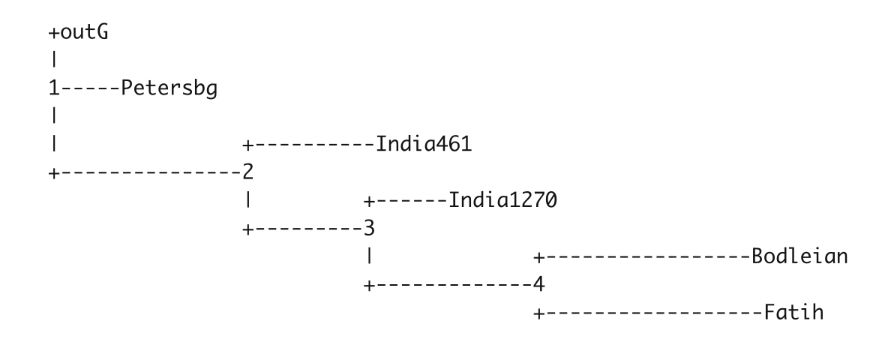
\includegraphics[width=\linewidth]{images/diagram_stemma.png}
	\end{subfigure}
	\hfill
	\begin{subfigure}{0.48\linewidth}
		\centering
		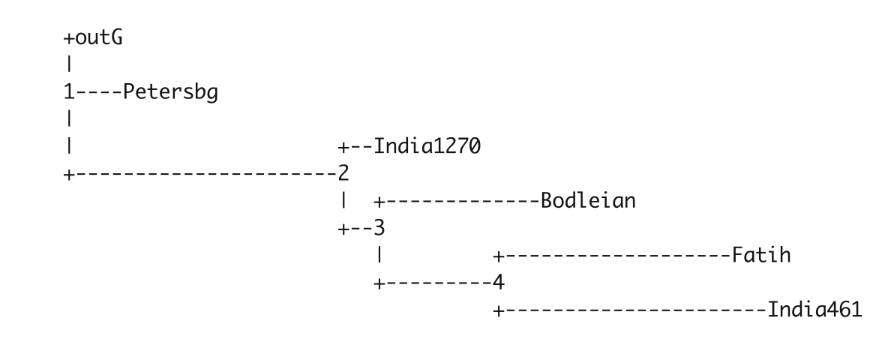
\includegraphics[width=\linewidth]{images/text_stemma.png}
	\end{subfigure}
	\caption{Stemmata pour les diagrammes (à gauche) et pour le texte (à droite) \footcite{raynaudBuildingStemmaCodicum2014}}
	\label{fig:stemma}
\end{figure}


En y regardant plus en détail, nous pouvons voir qu'il y a une forte similitude entre le \textit{stemma} textuel et le \textit{stemma} des diagrammes. Il en vient à la conclusion suivante : Quand les diagrammes sont intégrés au texte, il est envisageable de ne faire qu'un seul arbre pour les deux. Néanmoins, si les diagrammes ont été copiés a posteriori du texte ou qu'ils ont été corrigés par la suite, mieux vaut réaliser deux \textit{stemmata} distincts et étudier leur transmissions séparément. Le fait qu'ils aient été copiés par des personnes différentes à des moments différents impacte fortement leur étude. Il est même plus avantageux de réaliser le \textit{stemma codicum} d'une tradition mathématique à partir des diagrammes. La densité d'erreur serait sept à huit fois plus élevée dans un diagramme géométrique que dans un texte occupant la même superficie. Dans la mesure où sa méthode repose sur le relevé d'erreurs, il est plus judicieux de réaliser un \textit{stemma} avec des diagrammes\footcite{raynaudBuildingStemmaCodicum2014}.

Il nous est possible de retracer l'historique d'une œuvre grâce aux diagrammes. Cependant, ces derniers sont des éléments iconographiques complexes et il convient de les étudier de manière rigoureuse.

	\section{Limites des approches philologiques traditionnelles}
	L'historien des sciences \som{pas seulement} peut se heurter à de nombreuses difficultés lors de son étude des diagrammes. La manière de les représenter diffère en fonction des conventions et des choix éditoriaux. Comparer les diagrammes à l'œil nu devient complexe même pour un spécialiste. \som{Attention à la formulation, ce n'est pas forcément vrai et la comparaison manuelle sera toujours plus précise que le travail automatique.}

\subsection{Les différentes conventions de représentation d'un diagramme}

Le travail de l'historien des sciences peut s'avérer compliqué lorsqu'un concept ou une démonstration est représentée de manière différente dans différents témoins. \som{Non} En effet, les conventions et les choix graphiques des diagrammes diffèrent en fonction de l'époque, de l'endroit et du sujet d'étude.

Michela Malpangotto étudie ce phénomène en s'appuyant sur l'exemple de l'œuvre de Théodose les \textit{Sphériques} écrite au Ier siècle avant notre ère. Il s'agit d'un texte fondamental dans l'étude de la géométrie sphérique qui est structuré en cinquante-neuf propositions et divisé en trois livres. Il fait partie de ce que l'on nomme la \og Petite astronomie \fg, un recueil d'ouvrages compilés par les Grecs afin de faciliter la compréhension de l'\textit{Almageste} de Ptolémée. Il a été étudié et transmis pendant près de dix siècles. La géométrie sphérique est définie de la manière suivante : \og La géométrie sphérique étudie la sphère comme un objet solide mais surtout comme contexte spatial des éléments qui interagissent sur elle dans un agencement tridimensionnel complexe. \fg Il est alors nécessaire de mettre au même niveau, le plan du diagramme et l'agencement spatial des objets autour de la sphère. Cette dernière est un objet solide mais elle est surtout un contexte spatial pour des arcs, des segments de droites et des cercles qui y sont déterminés par l'intersection de différents plans inclinés dans l'agencement spatial tridimensionnel. Cependant, le concept de sphère n'est pas représenté de la même manière chez tous les auteurs \footcite{malpangottoGraphicalChoicesGeometrical2010}. 

Dans la version grecque originale, illustré ici par le manuscrit \textit{Vat. Gr. 204}, les deux parties de l'œuvre sont séparées par le choix de l'iconographie des diagrammes. Dans la première partie, nous retrouvons des diagrammes dans lesquelles la sphère n'est pas représentée. Il y a seulement des cercles produits par l'intersection du plan incliné de différentes façons qui sont représentés de manière juxtaposée dans le plan du diagrammes. Les arcs ainsi que les segments linaires sont aplatis et les objets placés de l'autre côté de la sphère sont retournés dans le plan de la figure. La conséquence majeure de ce mode de représentation est la dépendance des diagrammes vis-à-vis du texte. Il est nécessaire de lire les explications pour comprendre le diagramme. Dans la seconde partie de l'œuvre, les diagrammes sont construits en utilisant la perspective. Nous pouvons donc observer les éléments géométriques interagir entre eux à l'intérieur de cette dernière \footcite{malpangottoGraphicalChoicesGeometrical2010}.  

En Italie, Platon de Tivoli a réalisé trois éditions de cette œuvre au XVIe siècle en s'appuyant sur une version arabo-latine médiévale. Il choisit de représenter les diagrammes de manière schématique et plane comme dans la première partie de la version grecque originale de l'œuvre. L'édition de Francesco Maurolico marque un tournant dans la transmission des \textit{Sphériques}. En effet, ce dernier fait le choix de travailler sur la surface de la sphère qui, mise en avant, devient le contexte réel dans lequel les éléments géométriques interagissent. Christophe Clavius, un mathématicien allemand adopte cette iconographie dans son édition de 1586 qui sert de base à la tradition moderne des \textit{Sphériques}\footcite{malpangottoGraphicalChoicesGeometrical2010}. 

\begin{figure}[H]
	\centering
	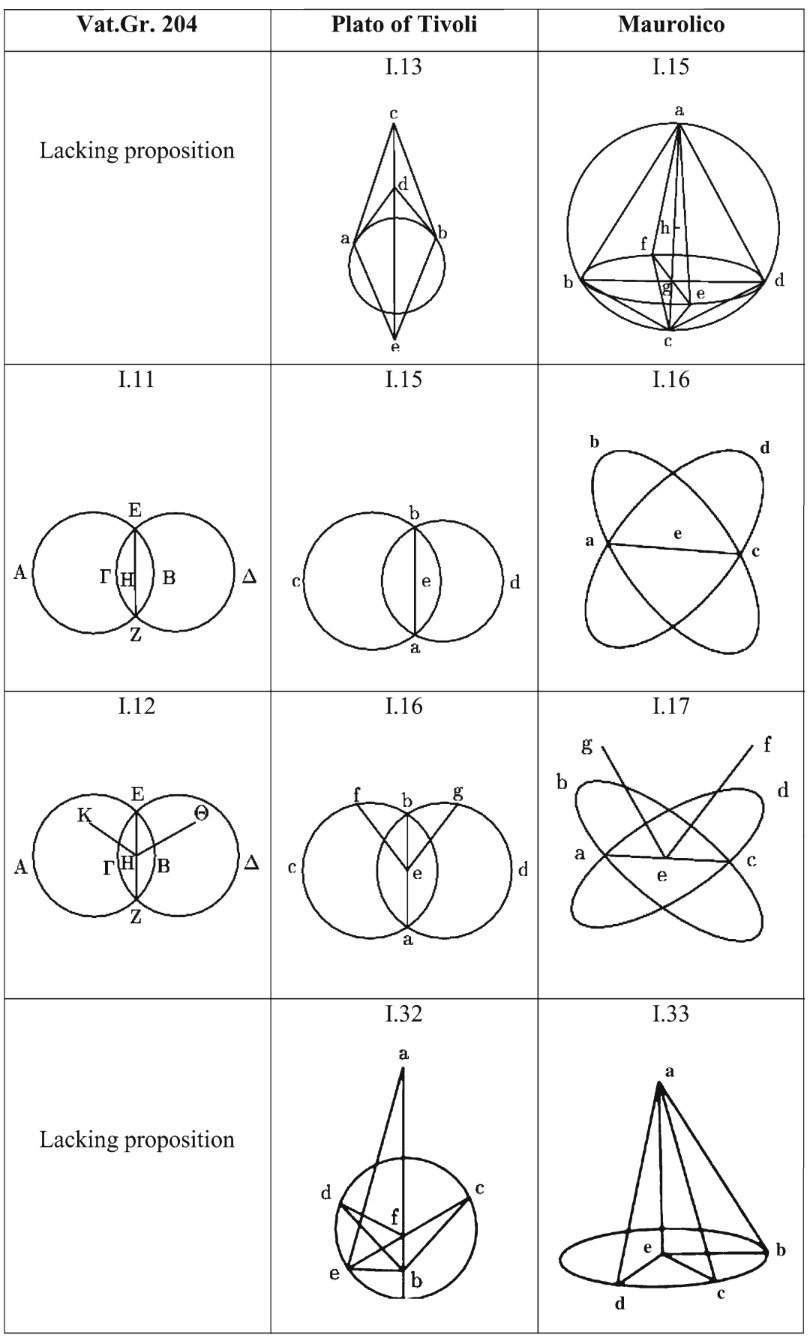
\includegraphics[width=0.6\linewidth]{images/conventions_diagrammes.png}
	\caption{Différentes conventions de représentation de diagrammes évoquées par Michela Malpangotto\footcite{malpangottoGraphicalChoicesGeometrical2010}}
	\label{fig:conventions}
\end{figure}


L'étude de Michela Malpangotto nous montre l'existence de nombreuses conventions graphiques de diagrammes pouvant être très différentes en fonction des éditeurs et des époques. Lorsque nous tentons de retracer la diffusion d'une œuvre à partir de ces diagrammes, il est important de prendre en compte ce paramètre. Néanmoins, ces différentes manières de représenter les diagrammes sont aussi en elles-mêmes les témoins de l'évolution d'un concept et donc par extension des connaissances scientifiques. \\

La question de la représentation des diagrammes est aussi une problématique que nous retrouvons dans les éditions plus contemporaines. 

\som{Mais du coup, les travaux cités comme exemple ont bel et bien été faits manuellement, sans que cela ne présente de difficulté particulière pour les chercheurs. Je pense que cette partie tombe à côté de la véritable problématique du projet, càd qu'il existe à travers les traditions un très grand nombre de manuscrits, qu'il est impossible sur le temps d'une vie de tous comparer précisément. De même, la question de la langue est importante, puisque c'est ça qui pose problème aux chercheurs qui sont rarement spécialistes de toutes les langues à la fois, et n'ont dans ce cas pas les outils pour faire des comparaisons à travers les traditions. Cela n'a rien à voir avec les conventions de représentation des diagrammes en elles-mêmes, d'autant qu'un outil numérique ne peut pas non plus faire cette comparaison automatiquement. On questionne donc la pertinence de l'argumentaire pour répondre à la problématique.}

\subsection{La modification des diagrammes dans les éditions modernes des sources scientifiques}

Les modifications que s'autorisent à faire les historiens et éditeurs contemporains peuvent rendre la comparaison avec les sources anciennes compliquée. Dans l'article déjà cité précédemment, Ken Saito étudie les éditions modernes des diagrammes astronomiques des \textit{Elements} d'Euclide. Il expose la problématique suivante : les diagrammes que nous voyons dans les éditions imprimées à partir du XIXe siècle sont très différents de ceux présents dans les manuscrits médiévaux. Pourtant les témoins datant du Moyen Age sont les meilleures versions, voire les seuls exemplaires d'œuvres antiques mathématiques en absence de manuscrit datant de cette époque. La version qui sert de base à beaucoup d'éditions contemporaines est celle de Heiberg datant de 1883-1888. Cependant, ce dernier s'est contenté de recopier les diagrammes de Ferdinand August simplifiés dans un but pédagogique dans son édition datant des années 1820 \footcite{saitoTraditionsDiagramTradition2012}. Se pose alors la question des conventions d'édition. Deux points de vue s'opposent. Nous avons d'abord celui de la maison d'édition \textit{Les Belles Lettres} décrit dans leur \textit{Règles et recommandations pour les éditions critiques} qui explique qu'il est nécessaire de reproduire les diagrammes aussi précisément que possible sans essayer de les corriger ou de les modifier. Michael Hunter, lui, défend plutôt l'idée selon laquelle il est acceptable que les diagrammes soient redessinés pour que l'intention originelle de l'auteur soit transmise au lecteur\footcite{jardineCriticalEditingEarlyModern2010}.\\

Ces différentes manières de représenter un même diagramme peuvent poser problème aux chercheurs lorsque ces derniers cherchent à établir des liens entre les différents témoins d'une même œuvre ou tradition. Même pour un spécialiste qui connaît parfaitement les différentes conventions, identifier et comparer chaque diagramme dans plusieurs témoins peut s'avérer être très chronophage.

\som{Pourquoi on voudrait comparer sources anciennes et contemporaines ? Ce n'est le sujet d'aucun projet de recherche cités dans le mémoire, et encore une fois, un chercheur qui le souhaite peut tout à fait faire cette comparaison. Ça n'a rien à voir avec les modifications que font les éditeurs et les historiens. Ce que AIKON/EIDA questionne, c'est l'absence de normes d'édition et de vocabulaire standardisé pour l'édition des diagrammes.}

	\clearemptydoublepage

	\chapter{AIKON et l'automatisation des traitements}
	\section{Le choix de la vision artificielle pour ces objets d'étude~: la plateforme AIKON}

	\section{Extraction de regions / Calcul de similarités}

	\section{De l'annotation manuelle au traitement de masse~: les interfaces existantes}

	\clearemptydoublepage

	\chapter{Vers la nécessité d'interfaces d'exploration}
	\section{Masse de données et limites de l'exploration manuelle}

	\section{De la correction d'annotations à l'interprétation scientifique}

	\section{Questions de recherche et besoins d'exploration du corpus}

	\clearemptydoublepage

	\part{Méthodologie de conception des visualisations exploratoires}
	\chapter{La visualisation en histoire}
	\section{Evolution des représentations visuelles en histoire}

	\section{Visualisations de réseaux et étude des disséminations}

	\section{Enjeux critiques de la médiation numérique des données historiques}

	\clearemptydoublepage

	\chapter{Formalisation des besoins et contraintes de conception}
	\section{Analyse des pratiques et questions des chercheurs EIDA}

	\section{Cahier des charges~: objectifs scientifiques et contraintes techniques}

	\section{Choix méthodologiques~: network graph et alignement des sources (bipartite)}

	\clearemptydoublepage

	\chapter{Processus itératif de développement}
	\section{Prototypage et tests de faisabilité technique}

	\section{Mise en oeuvre concrète~: choix techniques et difficultés rencontrées}

	\section{Intégration des retours utilisateurs et ajustements}

	\clearemptydoublepage

	\part{Évaluation critique et perspectives d'intégration}
	\chapter{Analyse des visualisations produites}
	\section{Visualisation bipartite~: révéler les réorganisations du contenu intellectuel}

	\section{Network graph~: explorer les chaînes de transmissions}

	\section{Adéquation aux objectifs d'exploration scientifique}

	\clearemptydoublepage

	\chapter{Validation et limites méthodologiques}
	\section{Critères d'évaluation de l'efficacité exploratoire}

	\section{Retour d'expérience par les chercheurs}

	\section{Limites liées aux données et biais d'interprétation}

	\clearemptydoublepage

	\chapter{Perspectives d'évolution et généralisation}
	\section{Intégration dynamique à la plateforme AIKON}

	\section{Transférabilité vers d'autres corpus et projets}

	\section{Implications pour l'évolution des pratiques en humanités numériques}

	\clearemptydoublepage

	\chapterNo{Conclusion}
	\addcontentsline{toc}{chapter}{Conclusion}

	\appendix
	\part*{Annexes}
	\addcontentsline{toc}{part}{Annexes}

	\clearemptydoublepage

	\backmatter
	\printacronyms[title=Liste des acronymes,toctitle=Acronymes]
	\printglossary
	\printbibliography
	\tableofcontents

\end{document}